\section{Facelift Framework}
We present here Facelift, an end-to-end  framework for
 image beautification. The framework embeds a model trained on a set of urban images annotated with beauty scores. It takes as input a geolocated urban image and gives as output its transformed (beautified) version. %The framework The current process concentrates for Beautification of urban images for the sake of this study, but the pipeline 
 Although we refer here to specific urban properties (i.e. beauty) and datasets, Facelift is generalizable to any labeled dataset of geolocated images. %The components work equally effective given that the principles of training a deep-learning model are followed. 
%We present here a pipeline for transforming natural geolocated images from one category to another. The current process concentrates for Beautification of urban images for the sake of this study, but the pipeline is generalizable for any annotated urban image dataset. The components work equally effective given that the principles of training a deep-learning model are followed. 

For the sake of berevity, we summarise the notations used in Table \ref{notations} and the pipeline steps in Figure \ref{fig:pipeline}. 
% \textbf{[add notations of T and R]}


\begin{table}[t]
	\resizebox{\linewidth}{!}{
		\begin{tabular}{l|p{8cm}}
			\textbf{symbol} & \textbf{stands for}\\
			$X$    & Georeferenced urban image dataset \\
			$I_i$    & Georeferenced image  $\in X $ \\
			$Y$    & Annotations classes for $X$ (e.g. beautiful/ugly)\\
			$y_i$    & Class in $Y$ (e.g. beautiful) \\
			$\hat{I_j}$ & Template image \\
			$I'$ & Target Image \\
			$C$ & Image Classifier \\
			$R$ & Images acquired by rotating street view camera \\
			$T$ & Images acquired by translating street view camera\\
			$\rho$ & Similarity bound below which smart augmentation chooses translated images \\
			& \\
			\textbf{term} & \textbf{stands for}\\
			\textit{Template Image} $\hat{I_j}$    & A synthetic transformation of input image $I$ towards the class $y_j$ \\
			\textit{Target Image} $I'$    & The natural image which is most visually similar to the template image \\
		%	\textit{ Data Clustering}    & A process which groups images in $X$ according to visual similarity (e.g urban vs rural)\\
			\textit{Data Augmentation}    & A process of data expansion which looks for images taken in the surroundings of the georeferenced images in $X$\\
			\textit{Classifier}   & A deep-learning framework that is able to classify images into one of the classes in $Y$\\
			\textit{Generator} $(GAN)$    & A deep-learning based image generator \\% framework to produce images similar to the ones in  $X$\\
			$DGN-AM$    & A framework that, given the GAN and the Classifier, transforms an input image into the template image.\\
	\end{tabular}}
	\caption{Notations and Terms.}\label{notations}
\end{table}

 \begin{figure*}[ht]
	\centering
	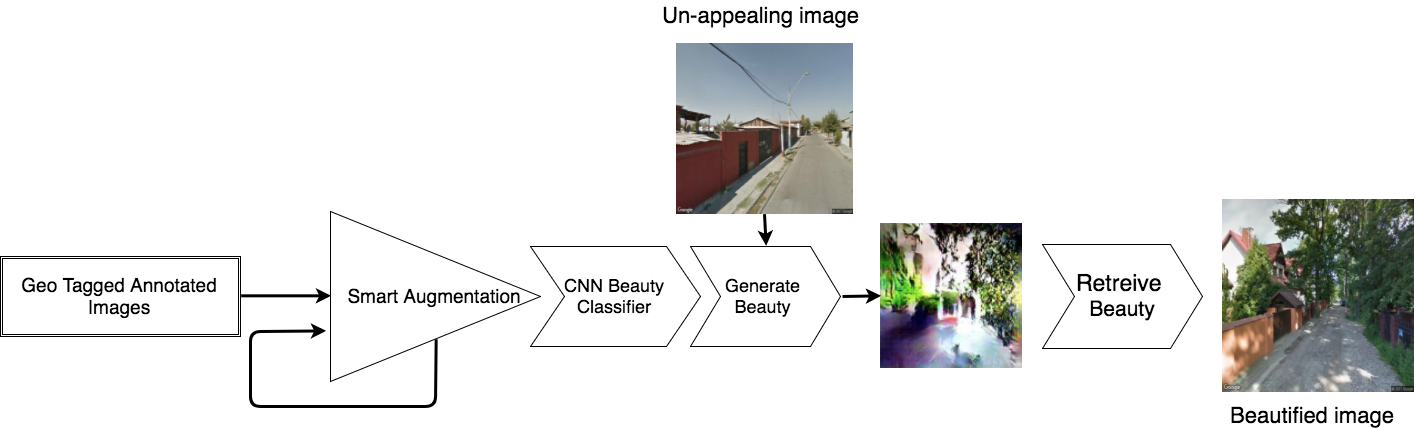
\includegraphics[width=2\columnwidth]{Plot/UrbanEmotionsPipeline.png}
	\caption{Architecture of the Beautification Pipeline}
	\label{fig:pipeline}
\end{figure*}

In general terms, the framework allows anyone with an arbitrary set of \emph{geolocated} images $ X = { I_1, I_2 ... . I_n  }$ annotated in classes $Y = {y_1 , y_2 , ... ,y_k}$, to transform natural images between classes: the algorithm can transform an  image $I_i$ belonging to class $y_i \in Y$ , to image $I_j$ from class $y_j \in Y$. Both $I_i$ and $I_j$ are natural, non-synthetic images. Despite having another \emph{meaning} (i.e. category), $I_j$ maintains the structural characteristics of $I_i$ (e.g. point of view, layout).  This allows  to visually reason about the discriminative properties between classes $y_i , y_j \in Y$, and visually understand the salient characteristics that drive a classifier to distinguish between  classes $y_i,y_j$. %The questions pertaining to what the network learns semantically have been explored for popular use cases \cite{mao2014explain,karpathy2015deep}  but still remain largely unexplored for intangible classes representing concepts like beauty, sentiment etc.  In this paper, we apply this general scheme to the specific problem of predicting beauty and explaining the changes that influence the beautification process. ---> TO RELATED WORK
\par 
The transformation framework consists of three phases (see Fig. \ref{fig:pipeline}). In the first phase, we classify images from $X$ into the corresponding categories $Y$ with high accuracy , using a convolutional neural network $C$. In our case, $y_i$  and  $y_j$ are the beautiful/ugly classes.
In the second phase, we transform am image from class $y_i$ to class $y_j$, using Generative Adversarial Networks\cite{radford2015unsupervised}. The output of this phase is a synthetic image $\hat{I_j}$, which summarizes the basic traits of the destination class $y_j \in Y$. The last phase matches the synthetic image $\hat{I_j}$,  with the closest natural image in $X$. Finally, to quantitatively reason about the beautification process, we perform aggregated analysis of the differences between original images and resulting target images.% matched natural image is then used to reason about urban design metrics that the network learnt to associate with beauty. 
We do this by quantifying the presence of 5 urban design metrics in uglified and beautified images.

For the rest of this section, we would delve deeper into the specifics of the image beautification framework. 

\subsection{Phase 1: Classifying Beauty}
We design here a classifier $C$  able to correctly assess the beauty category $y_i$ of an image in $X$ using a deep learning network. To reliably train a convolutional neural netowrk we need first make sure we have enough reliable data to train the classifier \textbf{[REF]}. We do this by augmenting the available geolocated image data. 

\subsubsection{Dataset and Beauty Judgements}
\label{sec:label}
Our seed dataset comes from Place pulse, a research work on urban affective dimensions \cite{dubey2016deep}. The dataset in total contains 100k images across 56 cities around the world from Google StreetView\footnote{https://maps.googleapis.com/maps/api/streetview}. Images are annotated through pair-wise comparison for qualities such as beauty, depression, richness , safety etc. For the purpose of our work, we use the beauty judgements. To train our classifier $C$ to detect beauty %in terms of 
categories $Y$, we need to transform pairwise votes into absolute scores, then discretize absolute scores into a finite set of categories $y_i$. We transform the pairwise votes %from the dataset are then transformed 
into ordinal scores using the TrueSkill \cite{herbrich2007trueskill} algorithm.  To ensure reliability of absolute judgements, we filter out images with less than 3 votes.
To discretize the resulting scores, we heuristically partition the data into two classes with maximum separation: beautiful and ugly. Figure \ref{fig:Trueskill} shows the distribution of Trueskill score estimates with the threshold scores at which we decide beauty or ugly class boundary. 

\begin{figure}[ht]
	\centering
	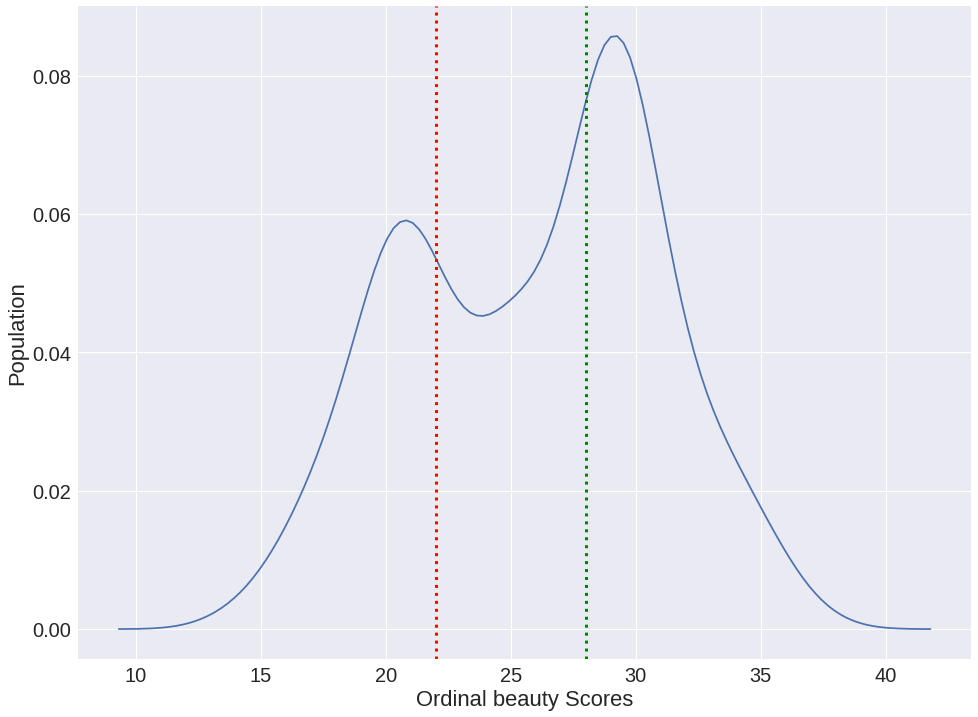
\includegraphics[width=0.7\columnwidth]{Plot/Trueskill.png}
	\caption{Distribution of ordinal scores for images with at-least 4 votes. The red and green line represent the threshold below and above which images are tagged Ugly or beautiful. Images in between are dropped for separability }
	\label{fig:Trueskill}
\end{figure}

\subsubsection{Data Augmentation similarity bound}
\label{sec:bound}
Despite over a hundred thousand images in the original data, only 20,000 has more than 3 judgements.
This is non-ideal to train classifiers with substantial number of parameters such as convolutional neural network,
since smaller data size implies that a machine learning model has a risk of over-fitting \textbf{[REF]}. We choose to augment the dataset by exploiting the geo-located nature of the image dataset. We also take advantage of the fact that urban places in close proximity look quite similar to each other \cite{parislooklikeparis}  
%\textbf{[There was a reference here from Daniele]}.
To develop a better way of augmenting images which can be transferred with scores of the original annotated ones, we make one heuristic assumption : "\textbf{[A1]}\textit{the composition of a StreetView image does not change considerably for small rotations of the camera angle}". This assumption was tried and tested over several samples both manually and using image similarity measures. An example of one such sample can be seen in Figure \ref{fig:rotSim}. This assumption allows us to do a basic expansion of our dataset without adding a lot of noise. However we cannot to a similar assumption when it comes to translation of camera. 
%we derive two new sets of augmented images. 
%\textbf{[Explain this assumption better - give example, refer to \ref{fig:rotSim} ]}.
%With an assumption that "\textbf{[A1]}\textit{rotation of camera, keeping the location constant, does not change the composition of the image considerably}" we now have two sets of images. 
All images in the PlacePulse dataset are taken with a default camera rotation which depends on the location. The Streetview API allows to specify the preferred camera rotation angle. This gives us the opportunity to take snapshots of the same location at different camera angles. We rotate the camera across different values $\theta \in {-30^{\circ}, -15^{\circ} , 15^{\circ} , 30^{\circ} }$ and derive a first set  $R=\{R(I)_{\theta} \forall I \in X\}$ , which consists of images acquired by rotating the camera angle for each annotated image in $X$. Following \textbf{A1}, For these images, the beauty score of each rotated image $R(I)_{\theta}$ can be safely transferred from $I$. 
%First set  is $R(I_i) \forall I_i \in X$ , which consists of images acquired b	y just rotating the camera angle for a given annotated image. We rotate the camera across different values $\theta \in {-30^{\circ}, -15^{\circ} , 15^{\circ} , 30^{\circ} }$. For these images, the beauty score can be safely transferred from $i$. 

Next, for each image in $X$, we translate the location of the Streetview camera: we select points on the map at a distance of $d \in \{10,20,40,60\}$ meters and acquire the resulting set of images $T=\{T(I)_d \forall I \in X\}$%, by translating the location of Streetview camera a near geographic vicinity of a StreetView image $I_i$ in $X$. We by translating the streetview  camera at distances of 10, 20 40 an,d 60 meters
. Although possibly very similar, transferring the beauty score from $I$ to each $T(I)_d$ might result in very noisy data. To understand the extent to which beauty scores can be transferred from images to their translated version, we use a smart augmentation technique. 


In a nutshell, this technique computes the similarity between the translated and the original image, and transfers the beauty scores only if the similarity is acceptably high.
To do so, we represent each images from both sets using visual features extracted from the FC7 layer of PlacesNet \cite{zhou2014learning}. We then calculate the cosine similarities $ S_t = \{s(I,T(I)_d) \forall I \in X \}$
between each original image $I$ and all images in the augmented set $T(I)_d$. 
We also calculate another set of cosine similarities  $ S_r = \{s(I,R(I)_{\theta}) \forall I \in X \}$ between rotated and origianl images. We define a similarity bound as the median similarity betwen rotated and original images.
\begin{equation}
\rho = median(S_r) \text{ where }{S_r} = \{s(I,R(I)_{\theta}) \forall I \in X \}
\label{eq:bound}
\end{equation}
Following the assumption \textbf{[A1]} , we only transfer beauty scores to translated images who look as similar to the original as their rotated counterparts: $s(I,T(I)_d) < \rho$. We discard translated images not fullfilling this requirement and retain the resulting images in the smartly translated image set $\hat{T}$. %namely only to those translated images whose similarity score to the original image  rotation of camera. 


%\begin{figure*}[ht]
%	\centering
%	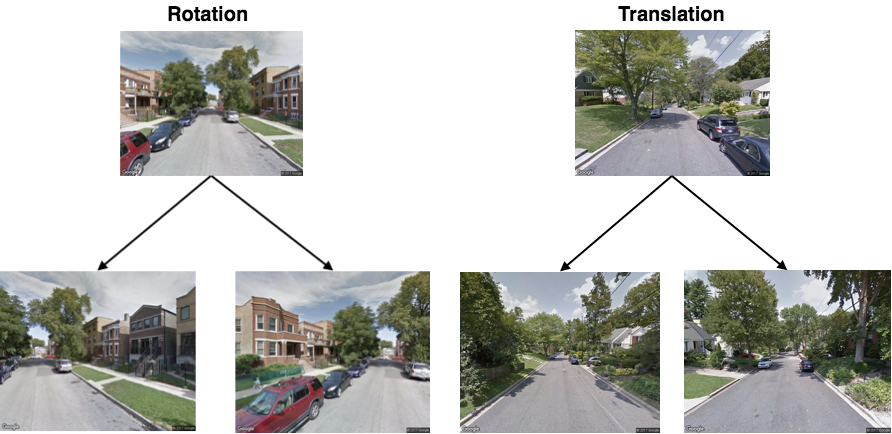
\includegraphics[width=1.25\columnwidth]{Plot/AugmentationExample.png}
%	\caption{Example images showing similarity of streetview scapes, when the camera is rotated by a small angle. The translational example shows similarity of images where the angle is less than the established bound $\rho$}
%	\label{fig:augmentationExample}
%\end{figure*}

\begin{figure*}[!t]
	\centering
	\hspace*{-5mm}
	\subfloat[]{
		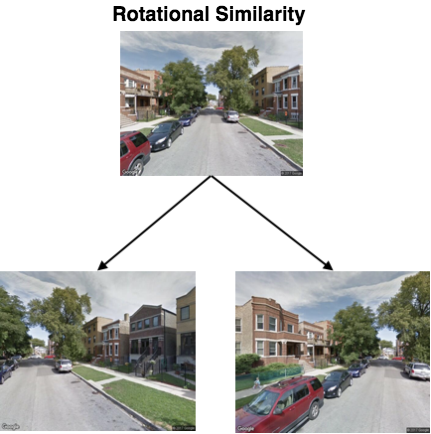
\includegraphics[width=0.3\textwidth, height = 5cm ]{Plot/rotationalSim.png}
		\label{fig:rotSim}
	}
	\subfloat[]{
		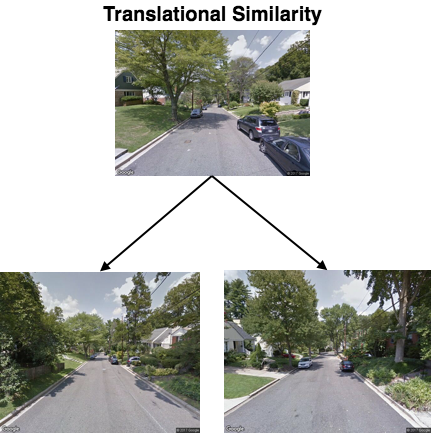
\includegraphics[width=0.3\linewidth, height = 5cm ]{Plot/transSim.png}
		\label{fig:transSim}
	}
	\vspace{-0.4cm}
	\caption{ Fig \ref{fig:rotSim} shows an example set of images showing similarity of streetview scapes, when the camera is rotated by a small angle. Fig \ref{fig:transSim} shows the translational similarity where the angle is less than the established bound $\rho$ }
	\vspace{-0.4cm}
\end{figure*}


\subsubsection{Semantics of Augmentable images}
Given that we now had a similarity bound to decide whether to augment or not a particular image, we wondered whether certain types of scenes are more prone to augmentation compared to others.  So we partitioned our data in two sets
\begin{itemize}
	\item $set A$: contains images where the median similarity  between translated images and the original image ${s(I,T(I)_d)} < \rho$ .
	
	\item $set B$:  Images whose similarity with their translated set is farther apart i.e. ${s(I,T(I)_d)} > \rho$ .
\end{itemize}

We describe each image in both sets according to the scene depicted, by collecting the PlacesNet \cite{zhou2014learning} labels with the top5 confidence scores. We then aggregate such labels at a set level by computing a TF-IDF metric. The resulting set of \{label,Count\} pairs reflect essentially how common or uncommon is a particular scene label in $setA$ compared to $setB$ 

\begin{figure}[ht]
	\centering
	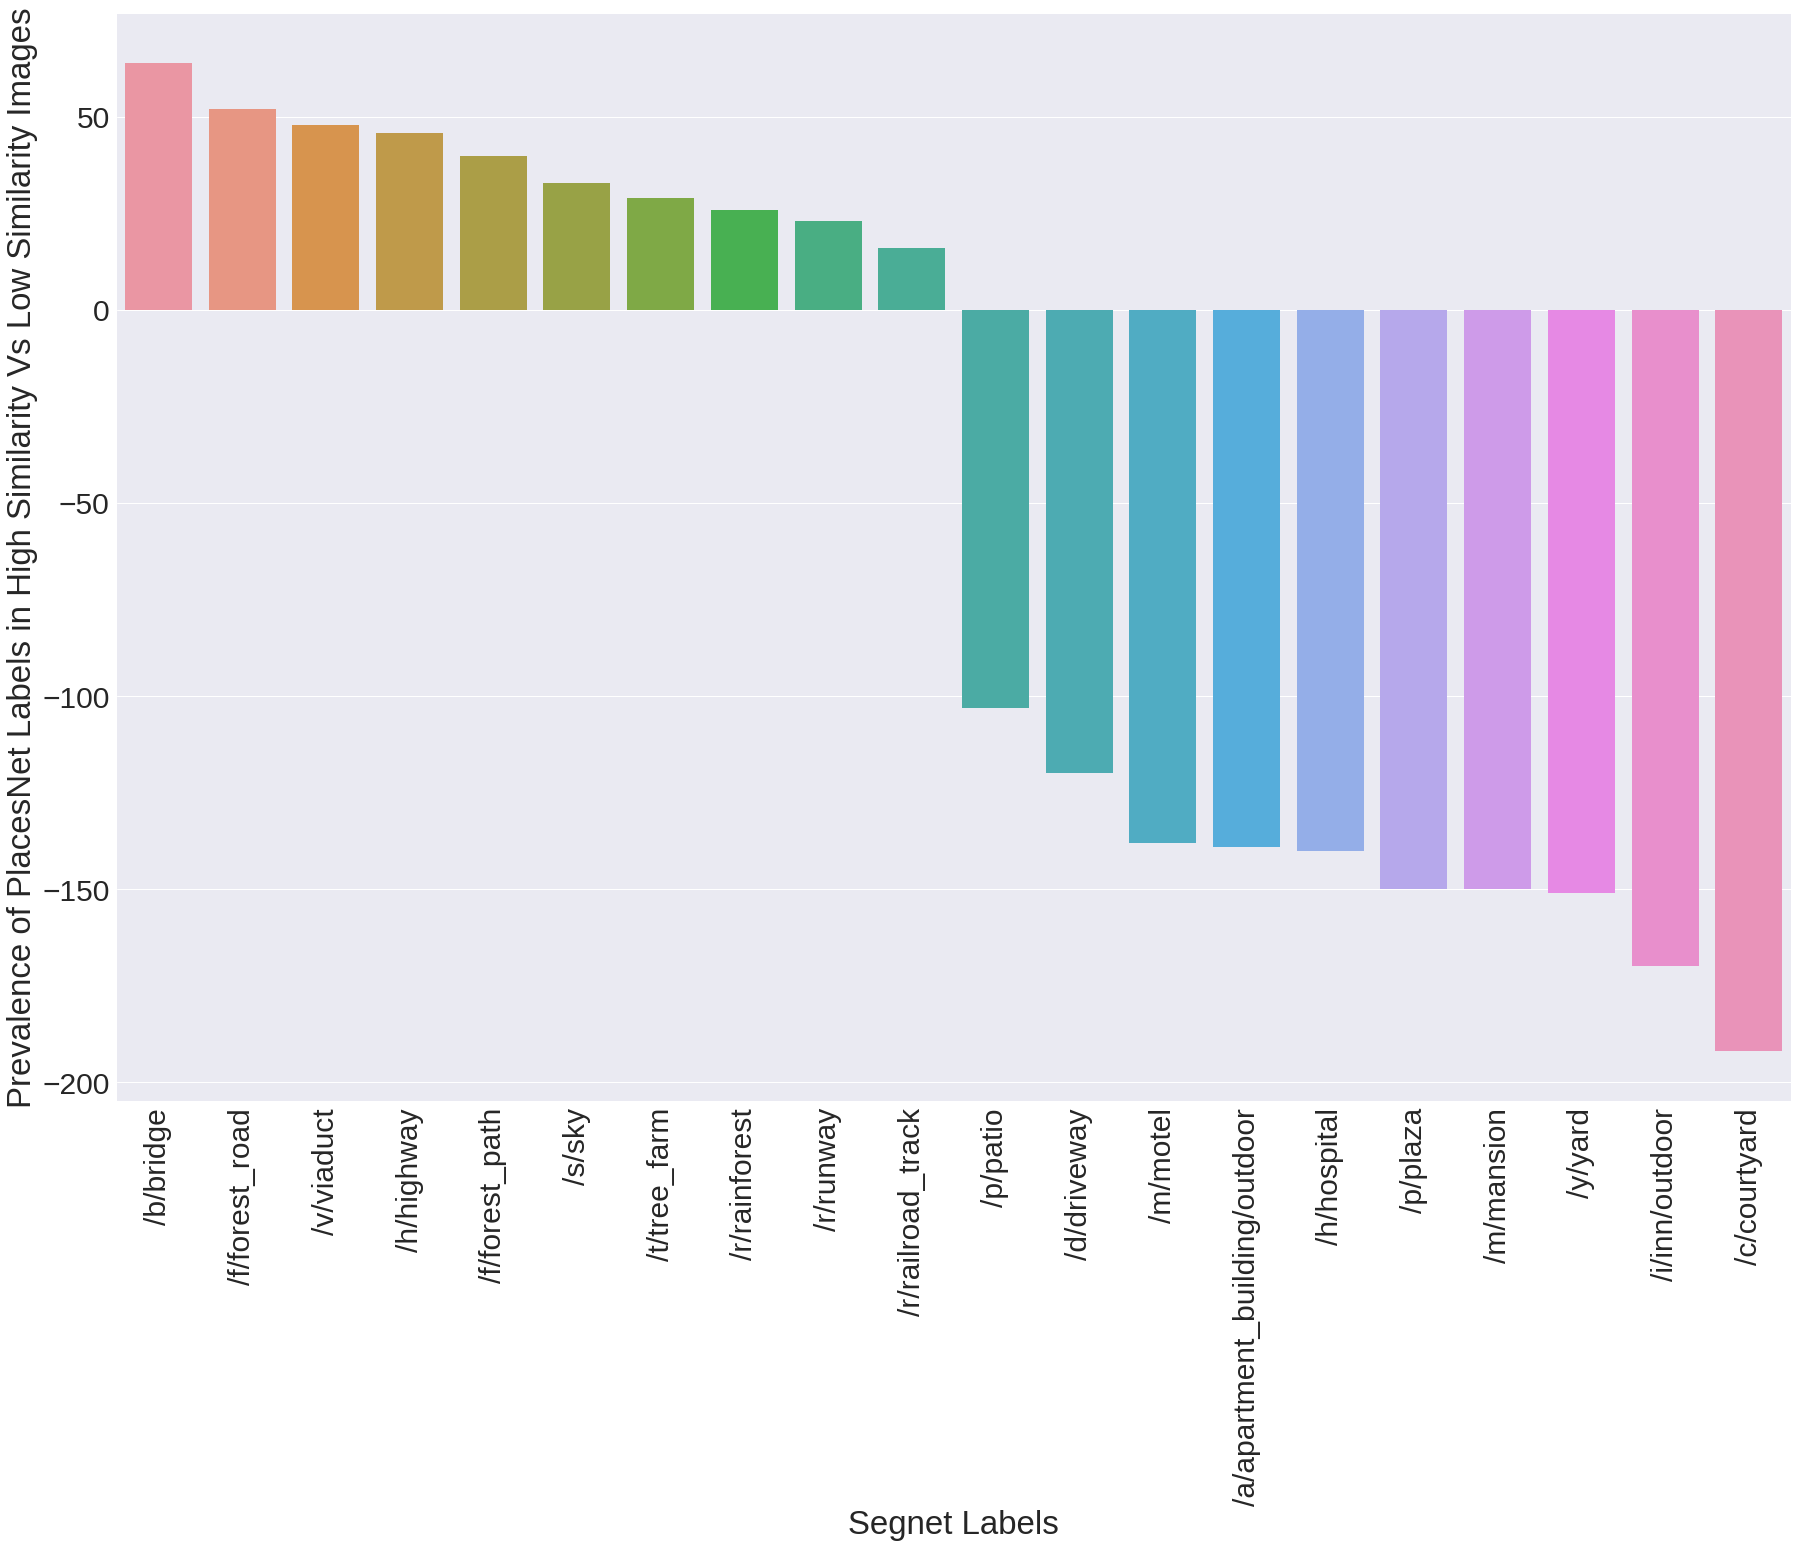
\includegraphics[width=\columnwidth]{Plot/SimilarityPlacesPrevalence.png}
	\caption{Prevalence plot of types of scenes prevalent in Similar images compared to dissimilar ones.}
	\label{fig:augmentationSimilarity}
\end{figure}

The resulting prevalences of scene types can be seen in Fig \ref{fig:augmentationSimilarity}. The plot shows that scenes like highways, fields and bridges, typically more uniform and open, 
don't change despite translation. Other urban scenes like gardens, residential neighbourhoods , plazas and skyscrapers  are more sensitive to change in perspective by translation. 


\subsubsection{The Beauty Classifier}
\label{sec:classifier}
Once we have enough data, we train a deep convolutional network %so as 
to classify images into the $Y$ beauty classes. One may use several successful deep convolutional neural network architectures, which work for other use cases like AlexNet \cite{krizhevsky2012imagenet} , PlacesNet \cite{zhou2014learning} or GoogLeNet \cite{szegedy2015going}.  For our paper we use CaffeNet which is a modified version of AlexNet. This trained classifier is a important component in the next phase, which is generation of images. 

We employ the above observations to train the beauty classifier model. We start with  the base dataset of 20k images ($X$), as described in Section \ref{sec:label}. We then progressively augment the data: first with rotation across 5 angles ($X$,$R$), then rotation with uniform translation for all images ($X$,$R$,$T$), and then rotation and translation for only images which satisfy similarity bound as evaluated as shown in Equation \ref{eq:bound} ($X$,$R$,$\hat{T}$). 
We then train a Convolutional neural net model based on AlexNet architecture \cite{szegedy2015going} on each of these augmentated datasets. The training is done on 70\% split of the data and tested on the 30\%. 

We see considerable improvement in classifier accuracy \ref{tab:classifier}, with the best model performing at 73\% accuracy for classifying images in two classes of Beauty and Ugly. 
This model represents the concept of beauty, learned from annotated and augmented streetview images. 


\begin{table}[h]
	\centering
	\begin{tabular}{|c|c|}
		\hline
		\textbf{Policy} & \textbf{Accuracy (Percentage)}\\
		\hline
		No augmentation ($X$) & 63 \\
		\hline
		Rotation only & 68 \\
		\hline
		Rotation + translation  & 64 \\
		\hline
		Rotation + Smart Translation & 73.5 \\
		\hline
		
		\hline
	\end{tabular}
	\caption{Performance differences based on different augmentation policies}
	\label{tab:classifier}
    \vspace{-10mm}
\end{table}



\subsection{Phase 2: Generating Images}
\par 
We now want to design a framework to transform any image $I_i$ of class $y_i$ into template image $\hat{I_j}$ (as shown in Figure \ref{fig:pipeline}), namely a synthetic version of the original image, with added features and motifs that maximize class $y_j$. 
To produce the template image $\hat{I_j}$, we need the following components in place:
\begin{itemize}
	\item {\textit{Classifier}}. We need a deep classifier $C$ able to classify $I$ into $Y$, i.e. between ugly and beautiful images. %This implies that it has learnt the abstract concept of beauty to some extent.
	
	\item \textit{Generator}. We train a generative adversarial network (GAN) which can generate an approximate natural looking image drawn from distribution of a particular class of images, similar to the one  in \cite{dosovitskiy2016inverting}. 
	
	\item \textit{Activation Maximization}. We plug in the GAN and the classifier network into an Activation Maximisation (AM) framework. Given these components, an input image $I$, and a target beauty class $y_i$, the AM transforms $I$ in an ideal image $\hat{I_j}$ ( that maximizes the activation for beauty class $y_i$).	
\end{itemize}
 
 We have described the design and performace of Classifier in Sec. \ref{sec:classifier}. We will delve deeper into the other two below
 
 \subsubsection{Generator}
 Generative Adverserial networks are an extremly useful tool when it comes to generating samples from a learned distribution\cite{radford2015unsupervised}. GANs consist of a %by learning a 
 pair of networks where the \textit{generator} %learns the distribution of sample space and 
 generates image samples similar to an input space using de-convolutional layers, and the \textit{discriminator} learns to discriminate between natural images from the training set and synthetic images generated by the generator. %The problem is a min-max arrangement where we want to maximize error in discriminator by minimizing error between generated and natural images, there by generating samples that confuse the discriminator. But 
Since GANs are known to be very tricky to train \cite{gulrajani2017improved}  we first try to use a pre-trained GANs on Imagenet from \cite{nguyen2016synthesizing}.However, because of the vast difference between images in Imagenet and Streetview images, our initial results were not very optimal. We therefore retrained the generator on the StreetScore dataset. %we used for Classification model. 
This improved the visual quality of the generated images considerably.%GAN performance considerably and it started generating images which do not entirely resemble natural streetview images, but look like paintings of these scenes. 

\subsubsection{Activation Maximization}

We build on top of the Activation Maximization technique elaborated by Nguyen et. al \cite{nguyen2016synthesizing} (DGN-AM). DGN-AM utilizes the property of locality of codes:% with respected to generated images in Generator networks. Which means G
Generator codes which are close to each other would create similar looking images. DGN-AM was initially built to visualise the concept learnt by CNNs, by finding the code which maximised the activation of a particular output class in the classifier network. %This approach was initially aimed at visualizing the learnt knowledge of a convolutional neural network classifier. This is done by maximizing the activation of a particular output class probability neuron in a trained Classifier network, by feeding it images generated by a generator network. 
The maximization is achieved by doing gradient descent on the input generator codes with respect to the classifier neuronal activation, keeping everything else locked. The result is a synthetic image that has a high activation for a pre-determined output neuron.
%\textbf{[Please modify the text below (please find in comment something taken from another paper ** PLEASE CHANGE ***)]}
We modify this method by starting the maximization method from a code $K$ which corresponds to the a-priori input image, for example, an ugly urban image $I_i$. So for a given image $I_i$ which belongs to class $y_i$ (which could be the beauty neuron or the ugly neuron of the classifier $C$), the DGN-AM algorithm would perform Stochastic gradient descent on the generator codes of the a-priori image $I_i$ so as to maximize the target neuron $y_j$ (which could be beauty of ugly neuron of $C$ resulting in a synthetic image $\hat{I}_j$ generated by the generator $G$ from the code $ \hat{K} $. The whole optimization can be expressed as Equation \ref{eq:dgn-am}.
 \begin{equation}
  \hat{I_j}=G( \hat{K} ) : \underset{\hat{K}}{\arg\max}(C_j(G(\hat{K}))-\lambda||\hat{K}||)
  \label{eq:dgn-am}
 \end{equation}
Here $C_j$ corresponds to the activation of the neuron $j$ of the classifier $C$ , and $G$ is the generator network. $\lambda$ is the $L_2$ regularization factor.
The resulting output image $\hat{I_j}$ is a natural-like image, which maximizes the beauty neuron for our classifier. We hypothesize that because the process begins from an a-priori image, the resulting image is closest possible template to the ugly input image, but with the beauty neural activation maximized. Figure \ref{fig:BeautyExample} shows the activation maximization output in the center.
%***HERE****
%Given an input image $i$, \emph{DGN-AM} iteratively re-calculates the color of $i$'s pixels in  a way  the output image $\hat{i}_h$  both maximizes  the  activation of neuron $h$ and looks ``photo realistic'',  which is done by conditioning the maximization to an ``image prior". This is equivalent to finding the feature vector $f$ that maximizes the following expression:
% \begin{equation}
%  \hat{i}_h=G( f ) : \underset{f}{\arg\max}(\Phi_h(G(f))-\lambda||f||),
% \end{equation}
% where:
% \begin{itemize}
% \item $G(f)$ is the image synthetically generated from the candidate feature vector $f$;
% \item $\Phi_h(G(f))$ is the activation value of neuron $h$ in the scene classifier $\Phi_h$ (the value to be maximized);
% \item $\lambda$ is a $L_2$ regularization term.
% \end{itemize}
% Here the initialization of $f$ is key. If $f$ were to be initialized with random noise, then the resulting $G(f)$ would be the average representation of category $h$ (of, e.g., a garden). Instead, since $f$ is initialized with $i$, then the resulting $G(f)$ is $i$'s morphed version. That is, the details that make $i$ distinguishable from other images of category $h$  are removed (e.g., the details that make $i$ distinguishable from images of gardens are removed). Overall, the result of the iterations is the image $G(f)$ whose look is close to the average representation of category $h$. 

%\begin{figure*}[h]
%	\centering
%	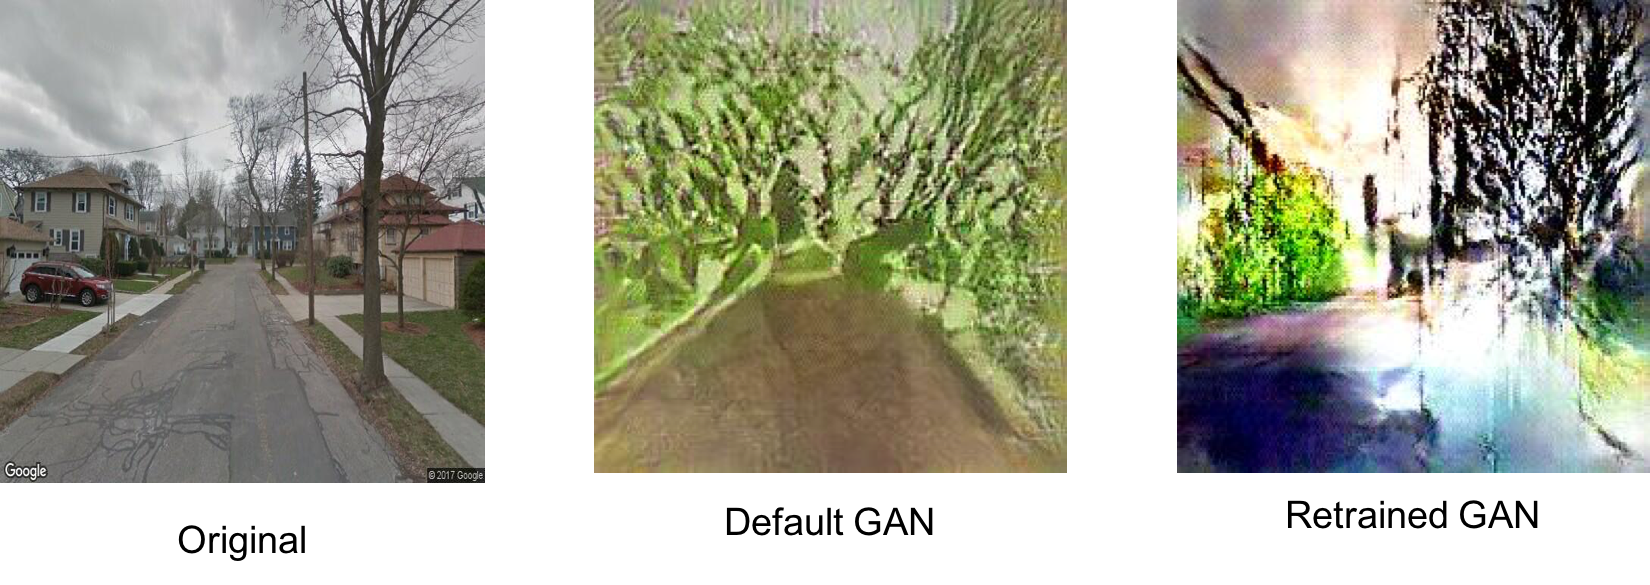
\includegraphics[width=0.7\linewidth]{Plot/GanCompare.png}
%	\caption{Comparison of using the Default ImageNet GAN against Custom trained GAN for Activation maximization. By re-training the GAN on the test dataset, we can see improvement in terms of structure and colours in the generated images}
%	\label{fig:GanComparison}
%\end{figure*}

\subsection{Phase 3: Retrieving Images }
%In mathematical terms, we want to choose a target image $I'$ from $X$ so as to minimize $E(I' , \hat{I_j} )$ , where $E(I_1, I_2)$ is some error measure that quantifies visual error between two images. This image $I'$ is effectively a natural transformed image.
In this final step we find a target image $I'$ from the dataset that is closely aligned, in terms of some visual similarity metric $E(I_1, I_2)$, with the generated template image  $\hat{I_j}$ . The result of this exercise is to find the most similar looking image to an input image $I$ that maximizes a particular annotation class $y_j$.
%The visual differences in these two natural images can act as the subject of reasoning for the explain-ability.
The problem of finding images which are visually similar can be solved using image embeddings in a $N$ dimensional space $R^N$
We use a pre-trained deep  network, which is trained to classify scene types to a very high accuracy \cite{zhou2014learning} to extract the image embeddings. We extract a 4096 dimensional feature vector from the FC7 layer of the network to describe the the template image. We then extract feature vectors from the complete test dataset using the same process. We can now use the $L_2$ Norm to find pairwise distances in the $R^{4096}$. Formally with $N$ test natural images and a template image $\hat{i}$ we extract $v_{\hat{i}} \in R^{4096}$ and and find pairwise distances  $\{d_j \text{  }\forall j \in N\} \text{ where } d_j = L_2(v_j , v_{\hat{i}})$ 
We then find the target image by finding the $min(\{d_j\})$. For the sake of redundancy, we find the top 5 such matches for every template $\hat{i}$ generated from every ugly image $i$. These target images are what we call the transformed images.

\begin{figure*}[h]
	\centering
	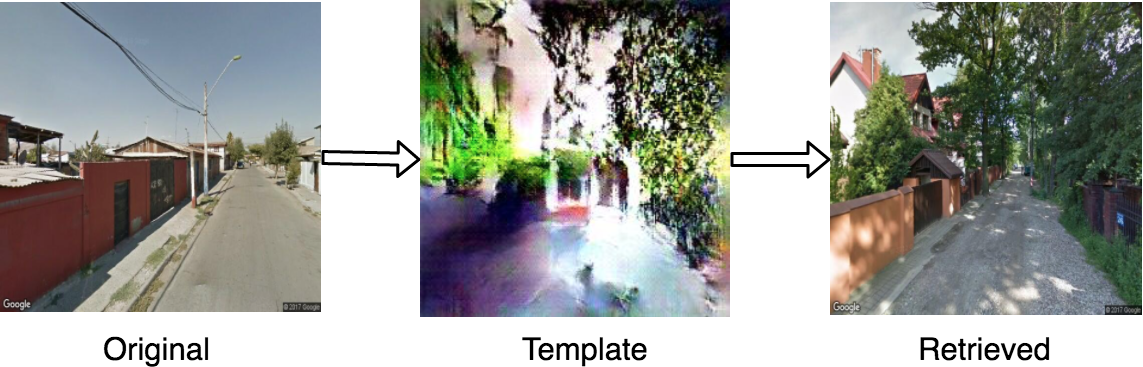
\includegraphics[width=0.5\linewidth]{Plot/Example.png}
	\caption{Example of Beautification Process}
	\label{fig:BeautyExample}
\end{figure*}

\subsection{Pipeline Validation}
%\textbf{[add EXP details! number of participants, agreement, pay, and ground truth construction ...]}
Because beauty is a subjective notion, we need to understand if our framework actually correctly transforms images into more or less perceptually beautiful. For this, we run a user study to check how often humans agree with the machines inference. We designa a  crowd-sourcing experiment to understand how much do real humans agree with the pipeline's transformations.
We randomly select 200 images, 100 beautiful  and 100 ugly as per their TrueSkill scores. To have a reliable seperation in terms of visual appeal, we only select ugly images with scores less than 15 and beautiful images with scores greater than 30. This means that we are selecting images from the bottom 10 and top 10 percentiles according to the Trueskill distribution as shown in figure \ref{fig:Trueskill}. These images are then transformed to the opposite side of the spectrum of beauty using FaceLift. As a result, a beautiful image would be transformed into an ugly image and vice versa. Then we design an Amazon Mechanical Turk experiment, where we ask the turkers to choose the beautiful image between the original and the transformed images, without giving any hints of the transformation. We pay 0.1\$ per human intensive task and we make sure that each Turker is a verified master, which assures that the Turker has a HIT approval rate above 90\% for the past 30 days. We make sure that we have at least 3 votes on each image comparison, there by allowing us to choose majority voting.The results show that over all , the Turkers agree with the model \textbf{77.5\%} of the times. Besides the overall agreement, the turkers agree \textbf{70\%} of the time with the process of beautification and \textbf{85\%} of the time with uglyfication. These results show that the facelift pipeline is learning the concept of beauty and then doing agreeable transformations on images.  